\documentclass[reprint,onecolumn,prb,superscriptaddress]{revtex4-2}
\usepackage{braket,amsmath,amssymb,graphicx,float,hyperref,color,ulem,soul,lipsum}
\allowdisplaybreaks
\bibliographystyle{apsrev4-2}
\begin{document}

\title{Supplementary Materials for ``Frustration shapes multi-channel Kondo physics: A star graph perspective"}

\author{Siddhartha Patra}
\email{sp14ip022@iiserkol.ac.in }
\affiliation{Department of Physical Sciences, Indian Institute of Science Education and Research-Kolkata, W.B. 741246, India}
\author{Abhirup Mukherjee}
\email{am18ip014@iiserkol.ac.in }
\affiliation{Department of Physical Sciences, Indian Institute of Science Education and Research-Kolkata, W.B. 741246, India}
\author{Anirban Mukherjee}
\email{mukherjee.anirban.anirban@gmail.com }
\affiliation{Department of Physical Sciences, Indian Institute of Science Education and Research-Kolkata, W.B. 741246, India}
\author{A. Taraphder}
\affiliation{Department of Physics, Indian Institute of Technology Kharagpur, Kharagpur 721302, India}
\author{N. S. Vidhyadhiraja}
\email{raja@jncasr.ac.in}
\affiliation{Theoretical Sciences Unit, Jawaharlal Nehru Center for Advanced Scientific Research, Jakkur, Bengaluru 560064, India}
\author{Siddhartha Lal}
\email{slal@iiserkol.ac.in}
\affiliation{Department of Physical Sciences, Indian Institute of Science Education and Research-Kolkata, W.B. 741246, India}
\date{\today}
\maketitle

\section{Additional Properties of the Star Graph}

\subsection{Energy lowering due to quantum fluctuations}
The star graph Hamiltonian that sits at the heart of the RG fixed point Hamiltonian of the multichannel Kondom model contains a classical Ising term and a quantum fluctuation term:
\begin{equation}\begin{aligned}
	H = {\mathcal{J}}\vec{S_d}\cdot\vec S = \mathcal{J}\left[\underbrace{S_d^z S^z}_\text{Ising term} + \underbrace{\frac{1}{2}\left(S_d^+ S^- + \text{h.c.}\right)}_\text{quantum fluctuation part} \right] = \mathcal{J}\left[\mathcal{H}^C + \mathcal{H}^Q\right] 
	\label{eq:stargraph_hamiltonian}
\end{aligned}\end{equation}
We are interested in studying how the presence of quantum fluctuations in the Hamiltonian of eq.~\ref{eq:stargraph_hamiltonian} stabilises the ground state. This can be understood by looking at the contributions, per channel, of the classical and the quantum parts to the total ground state energy \(E_g\). In the overscreened case \(\left( K > 2S_d \right) \), the contributions are
\begin{gather}
	E_{C} = \frac{1}{K}\langle \psi_g | \mathcal{H}^C | \psi_g \rangle, ~~~~~ E_{Q} = \frac{1}{K}\bra{\psi_g}\mathcal{H}^Q \ket{\psi_g} =\frac{E_g/\mathcal{J} - E_{C}}{K} =  -\frac{1}{2}S_d - \frac{1}{K}\left(S_d + E_{C}\right)
\end{gather}  
where we have defined the contributions \(E_C\) and \(E_Q\) to the ground state energy coming from the Ising and fluctuation parts respectively, and we have substituted the ground state energy \(E_g\) for the overscreened case {\color{blue}from the expression in the main text, just below where the star graph is introduced}. This contribution $E_Q$ is generated by the spin-flip fluctuations between the impurity spin and the outer spins of the star graph. Note that because of the degeneracy of the ground state subspace, there are multiple ground states characterised by different values of \(J^z = S^z + S_d^z\), and different ground states lead to different values of \(E_Q\).

The variation of \(E_Q\) is shown in Fig.\ref{fig:quantum_energy} for the case of $S_d=1/2$, as functions of the number of channels \(K\) as well as the ground state value \(J^z\) in which \(E_Q\) is being calculated. For a particular channel $K$, we find that the maximum \(|E_Q|\) is obtained for the state with smallest magnitude of $J^z$ (\(J^z = 0 \) for odd \(K\) and \(J^z = \pm 1/2\) for even \(K\)), whereas \(|E_Q|\) is minimum in the states with largest \(J^z\) ($J^z=\pm J$). The larger values of \(|E_Q|\) indicate that the quantum fluctuations are largest in the states with minimum \(J^z\), and these states can be thought of as the counterparts to the maximally entangled singlet seen in the single-channel Kondo problem. This behavior persists as \(K \gg 1\): the magnitude \(|Q_Q|\) associated with the $|J^z|= J$ states vanish, showing the classical nature of these states and the lack of quantum fluctuations in that limit. On the other hand, the state $|J^z| = |J^z|_{min}$ has a non-zero \(|E_Q|\) in the large \(K\) limit and hence contains some non-zero quantum fluctuations, showing the true quantum nature of this macroscopic singlet state.

\begin{figure}[!htb]
\centering
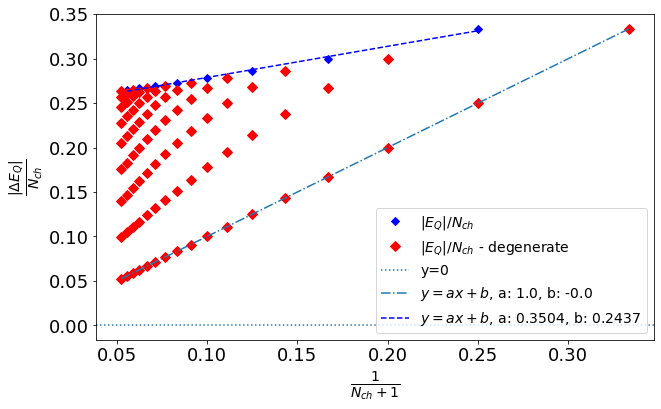
\includegraphics[width=0.7\textwidth]{plt/all/Quantum_Energy_per_channel}
\caption{This shows the variation of quantum energy per channel with $1/N$, where $N=N_{ch}+1$ is the total number of spins in the systems including the impurity spins. {\bf REMOVE DELTA IN YLABEL}}
\label{fig:quantum_energy}
\end{figure}

\subsection{Measure of quantum fluctuations}
Here we are interested in calculating the quantum fluctuation present in the  ground state by measuring the expectation value of the spin-flip part of the Hamiltonian: ${\mathcal{Q}}\equiv \langle \psi_g | (J^x)^2+(J^y)^2 |\psi_g\rangle = \langle \psi_g | J^2 - (J^z)^2 |\psi_g\rangle$. For a general spin-$S_d$ impurity, the ground state is characterised by $J=|K/2-S_d|$, which gives $J^2=J(J+1)=(|K/2-S_d|)(|K/2-S_d|+1)$. We define $\Delta=(K/2-S_d)$ to quantify the deviation from exact screening; $\Delta=0$ represents the exactly screened problem, and $\Delta>0$ and $\Delta<0$ represents the overscreened and underscreened problems respectively. Among the degenerate ground state, the maximum quantum fluctuation will occur in the state with minimum \(|J^z|\). Since \(J\) can actually be written as \(J = |\Delta|\), \(J\) will take integer values when \(\Delta\) is integer, and the minimum value of \(|J^z|\) is then zero. Otherwise, when \(\Delta\) is half-integer, \(J\) will also take half-integer values, and the minimum value of \(|J^z|\) is \(1/2\). With these considerations, the minimum value of the quantum fluctuation, {\it per channel}, is
\begin{equation}
q_K = \frac{1}{K}\sqrt{Q_\text{max}} = \frac{1}{K}\sqrt{\langle \psi_g | J^2 - |J^z|_{min}^2 |\psi_g\rangle} = \begin{cases}
	\frac{1}{K}\sqrt{(|K/2-S_d|)(|K/2-S_d|+1)-1/4}, & \text{ where }\Delta\text{ is half-integer}\\
	\frac{1}{K}\sqrt{(|K/2-S_d|)(|K/2-S_d|+1)}, & \text{ where }\Delta\text{ is integer}
\end{cases}
\end{equation}
This expression is symmetric under the transformation \(\Delta \to -\Delta\), and represents a duality between the overscrened and underscreend models. In the limit of large channel number \(K\), \(q_K\) simplifies to $\lim_{K\rightarrow \infty} q_K= \lim_{K \to \infty}\frac{1}{2K}|\Delta(K)|$. Only the over- and under-screened models have non-vanishing (and equal) values of \(q_K\).


\subsection{Staggerred magnetization of the star graph}
 Another probe to study the screening as a function of \(K\) is the staggered magnetization \(\vec{M}_s=\vec{S}-\vec{S}_d\). One can rewrite the Hamiltonian as $\vec{S}_d\cdot\vec{S}= \frac{1}{4}[J^2 - M_s^2]$. Since \(J\) and \(M_s\) commute with each other and hence also with the Hamiltonian, the eigenvalues of $\vec{J}^2$ and \(M_s^2\) act as good quantum numbers for in the ground states of the star graph model. The larger the value of \(\left<M_s^2\right>\), the stronger is the screening in that ground state. For single-channel case with $K=1$, the ground state is a unique 2-spin singlet $|\psi_g\rangle =\frac{1}{\sqrt{2}} (|\uparrow\downarrow\rangle-|\downarrow\uparrow\rangle = |J=0,J_z=0\rangle$, and the staggered magnetization per direction is \(M_s^2/3 = 1\), which shows the perfect screening.

Calculating the staggered magnetization for a general multichannel problem with \(K\) channels and a spin-\(S_d\) impurity reveals the breakdown of screening brought about by the presence of multiple channels. We find, in general, that the square of the staggered magnetization per channel is
\begin{equation}
	m_s^2 = \left< \left(\frac{1}{K}M_S\right)^2\right> = \frac{1}{K^2}\langle \psi_g | (\vec{S}_d - \vec{S})^2 |\psi_g\rangle = \frac{1}{K^2}\langle \psi_g | 2(\vec{S}_d^2 + \vec{S}^2)-\vec{J}^2 |\psi_g\rangle = \frac{2S_d(S_d+1)}{K^2}+\frac{1}{4}+\frac{1}{K}+\frac{1}{4K^2}
\end{equation}

\begin{figure}
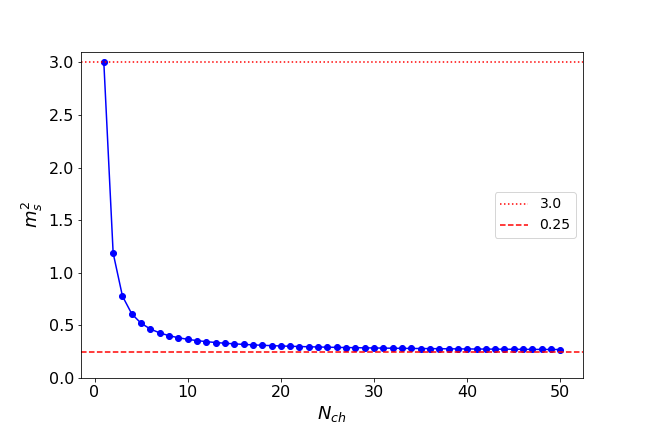
\includegraphics[width=0.7\textwidth]{plt/all/Staggered_mag_50.png}
\caption{This shows how the staggered magnetization changes with the number of channels $N_{ch}$.}
\label{fig:st_mag}
\end{figure}
This shows that as the number of channels increases, the value of \(m_s^2\) decreases from the perfectly-screened value of 3. For \(K \to \infty\) and keeping \(S_d\) finite, \(m_s^2\) approaches a lowered value of \(1/4\).

Due to the $SU(2)$ symmetry of the problem, the staggered magnetisation is the same along each of the three directions, such that the total value \(m_s^2\) is three times the value in any particular direction:
\begin{eqnarray}
\langle(m_s^x)^2\rangle=\langle(m_s^y)^2\rangle=\langle(m_s^z)^2\rangle=\frac{1}{3}m_s^2~,~~   
\end{eqnarray}
As mentioned above, the single channel case displays a value of $\langle (m_s^z)^2 \rangle =1$, showing the perfect screening. If one takes the limit of \(K \to \infty\) keeping \(S_d = K/2\), we get the staggered magnetisation at exact-screening and large \(K\), and the value is $\langle (m_s^z)^2 \rangle =1/4$. This is reduced from the value at \(K=1\). This reduced value however is still greater than the value of \(1/12\) reached as \(K\to \infty\) away from exact-screening by keeping \(S_d\) finite. These conclusions can be easily understood from fig.\ref{fig:st_mag} where we have shown the variation of \(\left<m_s^2 \right>\) as a function of \(K\), keeping \(S_d=1/2\).


\subsection{Thermodynamic quantitites}

\subsubsection{Impurity magnetization in terms of parity operators}
Just like the complete string operator \(\pi^z\), the modified string operator \(\sigma_d^z \pi^z\) is also a Wilson loop operator that wraps around only the outer nodes of the star graph:
\begin{equation}\begin{aligned}
	\pi^z_c \equiv \sigma_d^z \pi^z = \exp\left[i \frac{\pi}{2} \left(\sum_{l=1}^K \sigma^z_l - K\right)\right] 
\end{aligned}\end{equation}
The expectation value of the impurity magnetization along a particular direction and in specific ground states can be related to the 't Hooft operator. We will work in the state comprised of two adjacent eigenstates of \(J^z\):
\begin{equation}\begin{aligned}
	\ket{g^\theta_{J^z}} \equiv \frac{1}{\sqrt 2}\left( \ket{J^z} + e^{i\theta}\ket{J^z+1}\right), && J^z < \frac{1}{2}\left( K-1 \right)
\end{aligned}\end{equation}
The expectation value of the impurity magnetization operator \(\sigma_d^x\) can be expressed as
\begin{equation}\begin{aligned}
	\left<\sigma_d^x\right> \equiv \langle g^\theta_{J^z} \vert \sigma_d^x \vert g^\theta_{J^z}\rangle = - \langle J^z + 1 \vert \pi^x_c \vert -J^z \rangle + \text{h.c.}
\end{aligned}\end{equation}
This expression relates the observable impurity magnetization to the topological 't Hooft operator \cite{Maric2020}. Evaluating the matrix elements gives
\begin{equation}\begin{aligned}
	\label{sigmax}
	\left<\sigma_d^x\right> = - \frac{\sqrt{K^2 - (2J^z + 1)^2}}{2(1+K)}\cos \theta
\end{aligned}\end{equation}
Performing a similar calculation reveals that the impurity magnetizations along \(y\) and \(z\) in the same state are given by
\begin{equation}\begin{aligned}
	\label{sigmayz}
	\left<\sigma_d^y\right> = - \frac{\sqrt{K^2 - (2J^z + 1)^2}}{2(1+K)}\sin \theta, &&\left<\sigma_d^z\right> = - \frac{2J^z + 1}{(1+K)}
\end{aligned}\end{equation}
Combining eqs.~\ref{sigmax} and \ref{sigmayz}, we find
\begin{equation}\begin{aligned}
	\cos^2\theta\left(\left<\sigma^x_d\right>\right)^2 + \sin^2\theta\left(\left<\sigma^y_d\right>\right)^2 + \frac{1}{4}\left(\left<\sigma^z_d\right>\right)^2 = \frac{1}{4}\left(\frac{K}{1+K}\right)^2
\end{aligned}\end{equation}
This relation \textit{constrains the values of the magnetization} along all the directions: the \(x\) and \(y\) magnetization values have already been shown to be related to the `t Hooft operators \(\pi^x\) and \(\pi^y\) and the magnetization along \(z\) is therefore constrained in terms of the `t Hooft operators and the quantized function on the right-hand side (the function is quantized because \(K\) can only take integer values).

\subsubsection{Thermal entropy}
The star graph model can be solved to obtain the partition function, and this then allows the computation of the Helmholtz free energy and hence the thermal entropy:
\begin{equation}
\mathcal{F}= -k_B T\log Z, ~ ~ ~ S = -\frac{\partial \mathcal{F}}{\partial T} = -k_B \log Z -k_B T \frac{1}{Z} \frac{dZ}{dT} = -k_B \log \sum_{\epsilon} d(\epsilon) e^{-\beta \epsilon}  -\frac{1}{\beta} \frac{k_B\sum_\epsilon \epsilon d(\epsilon) e^{-\beta \epsilon} \beta^2   }{\sum_\epsilon  d(\epsilon)e^{-\beta \epsilon}}
\end{equation}
where \(d(\epsilon)\) is the degeneracy of the state at energy \(\epsilon\). The high and low temperature limits take very simple forms:
\begin{equation}
\lim_{\beta\rightarrow \infty} S = -k_B \log_2 d(\epsilon_{G})~,~~\lim_{\beta\rightarrow 0} S = -k_B \log \sum_\epsilon d(\epsilon)
\end{equation}

In fig.\ref{fig:thermal_entropy}, we plot the thermal entropy (in units of $k_B \log 2$) for a range of temperatures and for different values of \(K\). At large temperatures, \(S\) saturates to integer multiples of \(k_B \log 2\), while at low temperature, that is not always the case. This is because the total Hilbert space dimension \(\sum _\epsilon d(\epsilon)\) is simpy \(2^N\) (\(N\) being the total number of 1-particle states in the Hilbert space), and therefore \(\log \sum _\epsilon d(\epsilon) = N \log 2\) is always an integer multiple of \(N\). On the other hand, the ground state degeneracy \(d(\epsilon_G)\) is \(|K - 2 S_d|\) which is not necessarily of the form \(2^N\) and hence does not always lead to an integer multiple of \(\log 2\).

\begin{figure}
\centering
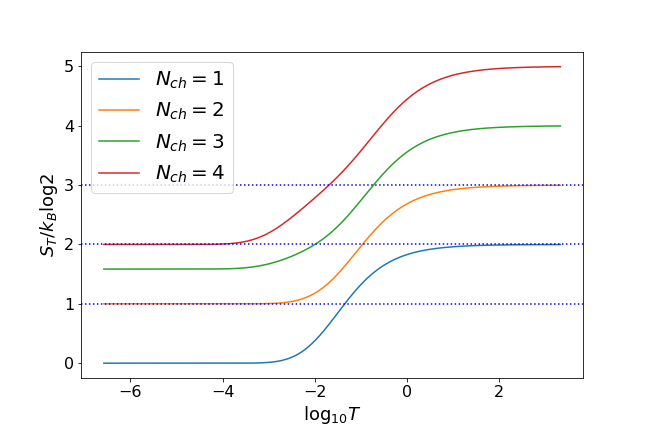
\includegraphics[width=0.7\textwidth]{plt/all/ThermalEntanglementVS_LogTemperature_}
\caption{This shows the variation of thermal entropy with the temperature.}
\label{fig:thermal_entropy}
\end{figure}

\section{Additional Topological Features of the Local Mott liquid}

The all-to-all Hamiltonian obtained by resolving the impurity-bath quantum fluctuations is written in terms of the spinor spin operators which are individually made out of two electronic degrees of freedom.
\begin{equation}\begin{aligned}
H_{eff} 
 =\frac{\beta_{\uparrow}({\mathcal{J}},\omega_{\uparrow})}{4} (S^+S^-+S^-S^+)   
\label{eq:all-to-all_1}
\end{aligned}\end{equation}
where \(\beta_{\uparrow} ({\mathcal{J}},\omega_{\uparrow})= ({\mathcal{J}}^2 \Gamma_{\uparrow})/2, ~ ~\Gamma_{\uparrow}=(\omega_{\uparrow}-{\mathcal{J}}(S_d^z-1))^{-1}\). This spin operator is defined as $\vec{S}_i=\frac{\hbar}{2} \displaystyle\sum_{\substack{ \alpha,\beta\in \{\uparrow,\downarrow\}}}  c_{0\alpha}^{(i)\dagger} \vec{\sigma}_{\alpha\beta} c_{0\beta}^{(i)}$. In the above eq.\eqref{eq:all-to-all_1} we see the $U(1)$ symmetry of the effective Hamiltonian. Using the spinor repersentation, we obtain the spin creation operation in terms of the electronic degree of freedom:
\begin{equation}
S_i^+ = \frac{\hbar}{2} \displaystyle\sum_{\alpha,\beta\in \{\uparrow\downarrow\}} c_{0\alpha}^{(i)\dagger} {\sigma}^{+}_{\alpha\beta} c_{0\beta}^{(i)}
=\frac{\hbar}{2} c_{0\uparrow}^{(i)\dagger} c_{0\downarrow}^{(i)}, ~ ~ ~S_i^z = \frac{\hbar}{2} \displaystyle\sum_{\alpha,\beta\in \{\uparrow\downarrow\}} c_{0\alpha}^{(i)\dagger} {\sigma}^{z}_{\alpha\beta} c_{0\beta}^{(i)} =\frac{\hbar}{2} (c_{0\uparrow}^{(i)\dagger} c_{0\uparrow}^{(i)} - c_{0\downarrow}^{(i)\dagger} c_{0\downarrow}^{(i)} )~,
\end{equation}
This spinor is simply the Anderson pseudospin formulation in the spin channel. The spin-creation opertor ($S_i^+$) involves the simultaneous creation of an electron-hole pair at the real space origin of the $i^{th}$ conduction channel. The condensation of such electron-hole pairs has already been shown in ~\cite{anirbanmott1,anirbanmott2}. Thus, for this effective Hamiltonian, one can define twist-translation operations to construct the gauge theory and unveil any hidden degeneracy.

Let's recall the effective Hamiltonian
\begin{eqnarray}
H_{eff} &=& \frac{\beta_{\uparrow}(\alpha,\omega_{\uparrow})}{4} \bigg[ \displaystyle\sum_{ij} S_i^+S_j^- ~+ \textrm{h.c.} \bigg]~,
\end{eqnarray}
where $i,j$ are the channel indices. Due to the all-to-all nature of the connectivity, one can draw a total of $K!$ possible unique closed paths ($\mathcal{C}_{\mu}$) such that each node (channel) is touched exactly once. These curves lead to $K!$ translation operators ($\hat{T}_{\mu}$) which keeps the Hamiltonian invariant. Let's define one such translation operator $\hat{T}_{\mu}=e^{i\hat{P}^{cm}_{{\mu}}}$ which gives a periodic shift along the closed path $\mathcal{C}_{\mu}$. The twist operator along the path $\mathcal{C}_{\mu}$ is given by
\begin{eqnarray}
\hat{\mathcal{O}}_{\mu} &=& \exp({i\frac{2\pi}{K} \displaystyle\sum_{\substack{j=1\\ \mathcal{C}_{\mu}}}^{K} j S_j^z} )~,
\end{eqnarray}
The action of the translation operator on \(S_j^z\) is to translate it by one channel index: $\hat{T}_{\mu} S_j^z \hat T^\dagger_\mu = S_{j+1}^z$ where $j+1$ and $j$ are the nearest neighbor on the closed path $\mathcal{C}_{\mu}$. Then the braiding rule between the twist and translation operators are give as
\begin{equation}
\hat{T}_{\mu}\hat{\mathcal{O}}_{\mu} \hat{T}^{\dagger}_{\mu} \hat{\mathcal{O}}_{\mu}^{\dagger} = \exp\{i[2\pi S_1^z-\frac{2\pi}{K}S^z]\} = \exp\{i[\pm \pi - \frac{2\pi}{K} S^z]\} =\exp(i\frac{2\pi p}{q})
\end{equation}
The availability of the non-trivial braiding statistics between these twist and translation operators is possible if $p\neq 0$ and $q\neq \infty$. Further simplification leads to the condition
\begin{equation}
 \pm\pi -\frac{2\pi}{K} S^z = \frac{2\pi p}{q} \implies  \pm\frac{1}{2}-\frac{S^z}{K} = \frac{p}{q} , ~ ~ ~ \frac{(\pm K-2S^z)}{2K} = \frac{p}{q}~,
\end{equation} 
where $p,q$ are mutual primes. We know that the $S^z$ can take values $(\mp K/2\pm m)$ where $m$ is a integer $0 \leq m \leq K$. Putting this value in the above equation leads to two possible solutions.
\begin{eqnarray}
\frac{(K-m)}{K} &=& \frac{p}{q} ~,~~ \frac{-m}{K}=\frac{p}{q}
\end{eqnarray}
For the first case $K-m=p$ we can see that $m=K$ makes $p$ trivial hus the allowed values are $m=0,\cdots,K-1$, which represents the corresponding $S^z$ eigenvalues 
\begin{eqnarray}
&&-K/2,-K/2+1,\cdots,K/2-2,K/2-1
\end{eqnarray}
Similarly the second case implies, $-m=p$, but $p=0$ is not allowed as this makes the braiding statistics trivial, thus the possible $S^z$ values are 
\begin{eqnarray}
&&\hspace{2.2cm} -K/2+1,-K/2+2,\cdots,K/2-1,K/2
\end{eqnarray}

Thus we get the general braiding statistics between the twist and the translation 
\begin{eqnarray}
\hat{T}_{\mu}\hat{\mathcal{O}_{\mu}} \hat{T}^{\dagger}_{\mu}\hat{\mathcal{O}_{\mu}}^{\dagger} &=& e^{i\frac{2\pi p}{K}}
\end{eqnarray}
where $p$ corresponds to different $S^z$ states, related as $p=\pm K/2-S^z$. Thus we can see that there are $K$ possible $S^z$ plaleau states in the all-to-all model where each plateaux is $K$ fold degenerate. This $p/K$ is similar to the filling factor of the fractional quantum Hall effect. There are possibly $K!$ pairs of twist and translation operator corresponding to different closed paths $\mathcal{C}_{\mu}$ which can probe this degeneracy.

\subsection{Action on the Hamiltonian}
We will now obtain the action of these twist operators on the Hamiltonian in eq.~\ref{eq:all-to-all_1}. Due the all-to-all nature of the effetive Hamiltonian one can find $K!$ possible relative arrangement of those $K$ channels which keeps the Hamiltonian invariant. Here we briefly discuss the choice of the closed loop $\mathcal{C}_{\mu}$ and the insertion of the flux. As shown in the {\color{blue}Fig.\ref{fig:stargraph-to-alltoall}(b)} we have chosen a particular closed path which crosses all the outer spin only once. We embed that closed loop on a plane and put the flux perpendicular to the plane through the closed loop. One can find a different closed loop where the ordering of the outer spins will be different. The action of the translation operator shifts the outer spins along this closed curve by one step.

\begin{figure}[htpb]
	\centering
	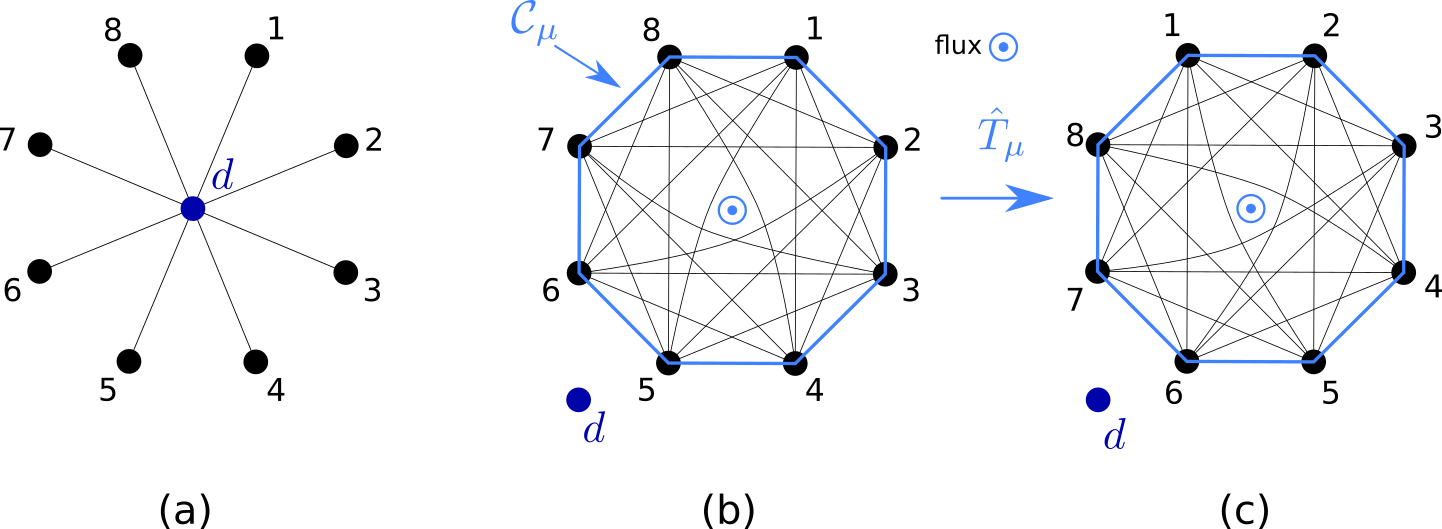
\includegraphics[width=0.8\textwidth]{./plt/stargraph-to-alltoall.png}
	\caption{(a) Schematic diagram of $8-$channel multichannel Kondo model zero mode in zero bandwidth limit. (b) All-to-all model obtained by disentangling the impurity spin from the bath zero modes. $C_{\mu}$ is a particular closed curve. (c) Translated configuration along the curve $C_{\mu}$ by one unit.}
	\label{fig:stargraph-to-alltoall}
\end{figure}

The action of the twist operator on the $S^x$ is determined in the follwoing calculation
\begin{equation}
\hat{O}_{\mu} S^x \hat{O}^{\dagger}_{\mu} = \exp({i\frac{2\pi}{K} \displaystyle\sum_{\substack{j=1\\ \mathcal{P}_{\mu}}}^{K} j S_j^z} )S^x \exp({-i\frac{2\pi}{K} \displaystyle\sum_{\substack{j=1\\ \mathcal{P}_{\mu}}}^{K} j S_j^z} ) = e^{X} S^x e^{-X}
\end{equation}
For simplicity of thte calculation we define $i\frac{2\pi}{K}=\Omega$, thus $X=\Omega\sum_j jS^z_j$. Thus we get
\begin{equation}
e^X S^x e^{-X}= S^x+[X,S^x] + \frac{1}{2!}[X,[X,S^x]] +\cdots = \sum_l ( S^x_l \cos \theta_l -  S_l^y \sin \theta_l ) ~,~~~\theta_l=\frac{2\pi l}{K}\\
e^X S^y e^{-X}= \sum_l  (S^y_l \cos\theta_l  + S^x_l \sin\theta_l)
\end{equation}
As already defined, $\theta_l=\frac{2\pi l}{K}=\frac{2\pi (K-n)}{K}$, where $n$ is an integer. We can see that in the large channel limit $\theta_l $ becomes inter multiple of $2\pi$. Thus in the large channel limit
\begin{gather}
 \lim_{K\rightarrow \infty}\hat{\mathcal{O}}_{\mu} H_{eff} \hat{\mathcal{O}}_{\mu}^{\dagger}\nonumber = \frac{\beta_{\uparrow}(\alpha,\omega_{\uparrow})}{2} \bigg[ \hat{\mathcal{O}}_{\mu} S^x \hat{\mathcal{O}}_{\mu}^{\dagger} \hat{\mathcal{O}}_{\mu} S^x \hat{\mathcal{O}}_{\mu}^{\dagger}  + \hat{\mathcal{O}}_{\mu} S^y \hat{\mathcal{O}}_{\mu}^{\dagger} \hat{\mathcal{O}}_{\mu} S^y \hat{\mathcal{O}}_{\mu}^{\dagger}  \bigg] = \frac{\beta_{\uparrow}(\alpha,\omega_{\uparrow})}{2} \bigg[  S^{x2}+S^{y2}  \bigg] = H_{eff},\\
 \lim_{K\rightarrow \infty } [\hat{\mathcal{O}},H_{eff}] = 0
\label{eq:hamiltonian_twisted}
\end{gather}
 
The translation operator $\hat{T}_{\mu}=e^{i\hat{\mathcal{P}}_{\mu}}$ commutes with the Hamiltonian, and hence the generator $\hat{\mathcal{P}}_{\mu}$ also commutes with the Hamiltonian. We can label the $j^{th}$ state with the eigenvalues of this operator $\hat{\mathcal{P}_{\mu}}$ as $|p^{j}_{\mu}\rangle$. The action of these twist and translation operators on these states are
\begin{gather}
\hat{T}_{\mu} |p^j_{\mu} \rangle = e^{i\hat{\mathcal{P}}_{\mu}} |p^j_{\mu} \rangle = e^{ip^j_{\mu}} |p^j_{\mu}\rangle, ~ ~ ~ ~ \hat{T}_{\mu} \hat{\mathcal{O}}_{\mu} |p^j_{\mu} \rangle =  \hat{\mathcal{O}}_{\mu} \hat{T}_{\mu} e^{i\frac{2\pi m}{K}} |p^j_{\mu}\rangle = \hat{\mathcal{O}}_{\mu}   e^{i(\frac{2\pi m}{K}+p_{\mu}^j)} |p^j_{\mu}\rangle~,~~ \frac{2\pi m}{K} \equiv p_{\mu}^{m} \\
\hat{T}_{\mu} \bigg( \hat{\mathcal{O}}_{\mu} |p^j_{\mu} \rangle  \bigg) = e^{i(p_{\mu}^{m}+p_{\mu}^j)} \bigg( \hat{\mathcal{O}}_{\mu}    |p^j_{\mu}\rangle \bigg)    
\end{gather}
where $m$ represents different $S^z$ plateaux. This shows that  $\hat{\mathcal{O}}_{\mu} |p^j_{\mu} \rangle $ is again an eigenstate of the translation operator, but with an eivenvalue that is different from $|p^j_{\mu} \rangle $, and is thus orthogonal to $\ket{p^j_{\mu}}$. Simiarly one can generally show that $\langle p^j_{\mu} | \hat{\mathcal{O}}^{q}_{\mu} |p^j_{\mu} \rangle=0$, where $q$ is any integer. Also in the large $K$ limit we can see from the eq.\eqref{eq:hamiltonian_twisted} that these differnt twisted states has same energy. Which shows that at each plateau state labeled by the $S^z$ eigenvalue has $K$ fold degenerate eigenstates labeled by the eigenvalue of the translation operators. The complete set of commuting observables is therefore formed by $H,S^z,\hat{T}$, and states can be labeled as  $|E,S^z_j,P^j_{\mu}\rangle$. 




\section{Effect of conduction bath excitations on the fixed point theory}
\subsection{Non-Fermi liquid signatures in momentum space for 2-channel Kondo}
Obtaining the effective Hamiltonian involves obtaining the low energy excitations on top of the ground state of the star graph. The large-energy excitations are ones that involve spin flips. This guides the separation of the Hamiltonian into a diagonal and an off-diagonal piece:
\begin{align}
	H = H_d + V = \underbrace{H_0 + J S_d^z s_\text{tot}^z}_{H_d} + \underbrace{\frac{J}{2}S_d^+ s_\text{tot}^- + \text{h.c.}}_{V + V^\dagger}
\end{align}
We define \(V\) as the interaction term that decreases \(s_\text{tot}^z\) by 1: \(V \ket{s_\text{tot}^z} \to \ket{s_\text{tot}^z - 1}\). Similarly, we define \(V^\dagger \ket{s_\text{tot}^z} \to \ket{s_\text{tot}^z + 1}\). The Schrodinger equation for the ground state can be written as
\begin{widetext}
\begin{align}
	E_\text{gs}\ket{\Psi_\text{gs}} = H \ket{\Psi_\text{gs}} = \left(H_d + V\right)\ket{\Psi_\text{gs}} \implies \left(E_\text{gs} - H_d\right)\sum C_{S_d^z, s_\text{tot},s_\text{tot}^z}\ket{S_d^z, s_\text{tot}, s_\text{tot}^z} = V\sum C_{S_d^z, s_\text{tot},s_\text{tot}^z}\ket{S_d^z, s_\text{tot}, s_\text{tot}^z}
\end{align}
\end{widetext}
\(E_\text{gs}\) is the ground state energy, and can be replaced by the star graph ground state energy if we remove the kinetic energy cost via normal ordering: \(E_\text{gs} = -\frac{J}{2}\left(\frac{K}{2}+1\right) \). Since the interaction part \(V\) only changes \(S_d^z \to -S_d^z\) and \(s^z_\text{tot} \to s^z_\text{tot} \pm 1\), we can simplify the equation into individual smaller equations. For the state \((s_\text{tot},s^z_\text{tot}) = (1,0)\), equations are
\begin{align}
	\label{eff_ham_Sdz_10}
	E_\text{gs} \ket{\frac{1}{2}, 1, 0} &= \left(H_d + V \frac{1}{E_\text{gs} - H_d}V^\dagger\right) \ket{\frac{1}{2}, 1, 0}\\
	E_\text{gs} \ket{-\frac{1}{2}, 1, 0} &= \left(H_d + V^\dagger \frac{1}{E_\text{gs} - H_d} V\right) \ket{-\frac{1}{2}, 1, 0}\\
\end{align}
These equations represent the Schrodinger equation for the states \(\ket{S_d^z, 1, 0}\), and the right hand sides therefore give the effective Hamiltonians for those states. If we combine the states into a single subspace \(\ket{1,0}= \left\{\ket{\frac{1}{2}, 1, 0}, \ket{-\frac{1}{2}, 1, 0}\right\}\), the effective Hamiltonian for this composite subspace becomes the sum of the two parts:
\begin{align}
	\label{eff_ham_10}
	H^{1,0}_\text{eff}\ket{1, 0}\bra{1, 0} = \left(H_d + V G_0 V^\dagger + V^\dagger G_0  V\right) \ket{1, 0}
\end{align}
where \(G_0 = \left(E_\text{gs} - H_d\right)^{-1}\). To calculate these effective Hamiltonians, we will expand the denominator in powers of in \(H_0^n/J^{n+1}, n=0,1,2,\ldots\). Expanding up to \(n=2\) and keeping at most two particle interaction terms, 
the effective Hamiltonian is
\begin{widetext}
\begin{align}
	H_\text{eff}^{1, 0} &= H_0 + \frac{J^2}{2\left(E_\text{gs} + \frac{J}{2}\right)}\left[1 + \frac{ H_0 + \left(\frac{1}{2} + S_d^z\right) s^+_\text{tot}X_{1,\text{tot}} - \left(\frac{1}{2} - S_d^z\right) s^-_\text{tot}X^\dagger_{1,\text{tot}}}{2 \left(E_\text{gs} + \frac{J}{2}\right)} + \frac{H_0^2}{\left(E_\text{gs} + \frac{J}{2}\right)^2} - \frac{Z_{1,\text{tot}} H_0}{\left(E_\text{gs} + \frac{J}{2}\right)^3} \right]
\end{align}
\end{widetext}
We employed the definitions 
\begin{equation}\begin{aligned}
X_{n,\text{tot}} \equiv  \sum_l \sum_{k,k^\prime}\left(\epsilon_k - \epsilon_{k^\prime}\right)^n c^\dagger_{k \downarrow}c_{k^\prime \uparrow}, ~ ~ ~ Z_{1,\text{tot}} \equiv \sum_{k,k^\prime,l}\left( \epsilon_k - \epsilon_{k^\prime} \right) \frac{1}{2}\left(c^\dagger_{k \uparrow,l}c_{k^\prime \uparrow,l} - c^\dagger_{k \downarrow,l}c_{k^\prime \downarrow,l}\right)
\end{aligned}\end{equation}
There are several non-Fermi liquid terms of the form \(s^+_\text{tot}X_{1,\text{tot}}, s^-_\text{tot}X^\dagger_{1,\text{tot}},Z_{1,\text{tot}} H_0\). These arise because of the degenerate manifold and the increased availability of states in the Hilbert space for scattering, as compared to the unique singlet ground state of the single-channel Kondo model.


\subsection{Low temperature thermodynamic behaviour}
The non-Fermi liquid (NFL) nature of the effective Hamiltonian can be demonstrated through a calculation of certain thermodyanmic quantities like the impurity specific heat and the magnetic suseptibility. We begin by calculating the self energy of this NFL hamiltonian. In real space one can extract a diagonal piece from the effective Hamiltonian by using the fermionic anticommutation relations.
\begin{eqnarray}
H_{eff}^{off,(2)} |_{diag} &=& -(16t^2/3) [ (S_1^z)^2+ (S_2^z)^2 ] 
\end{eqnarray}
the corresponding momentum space Hamiltonian is obtained from the fouries transform:
\begin{equation}
H_{eff}^{off,(2)} |_{diag}= -\frac{4t^2}{3} \frac{1}{N} \bigg[ \displaystyle\sum_{k,\sigma} n_{k\sigma}(1-\frac{1}{N} \displaystyle\sum_{k_2}  n_{k_2,-\sigma}  ) + \displaystyle\sum_{k,\sigma} \tilde{n}_{k\sigma} ( 1-\frac{1}{N} \displaystyle\sum_{ k_2} \tilde{n}_{k_2,-\sigma}  ) \bigg]  
\end{equation}
The above relation leads to the self-energy correction to the kinetic energy, which is
\begin{equation}
\bar{\epsilon} _k-\epsilon_k = \Sigma_k = -\frac{4t^2}{3N^2}\bigg(1-\frac{N}{e^{(\epsilon_k-\mu)/k_BT}+1}\bigg)
\label{eq:self-energy-NFL}
\end{equation}
Using the self-energy we calculate the impurity speciftic heat defined as $C_{imp}=C(J^*)-C(0)$ which is defined as
\begin{eqnarray}
C_{imp} &=& \sum_{\Lambda,\sigma} \beta \bigg[ \frac{(\bar{\epsilon}_{\Lambda})^2 e^{\beta \bar{\epsilon}_{\Lambda}}}{( e^{\beta \bar{\epsilon}_{\Lambda}} +1)^2}  -\frac{({\epsilon}_{\Lambda})^2 e^{\beta {\epsilon}_{\Lambda}}}{( e^{\beta {\epsilon}_{\Lambda}} +1)^2} \bigg]
\end{eqnarray}
\begin{figure}[!htb]
\centering
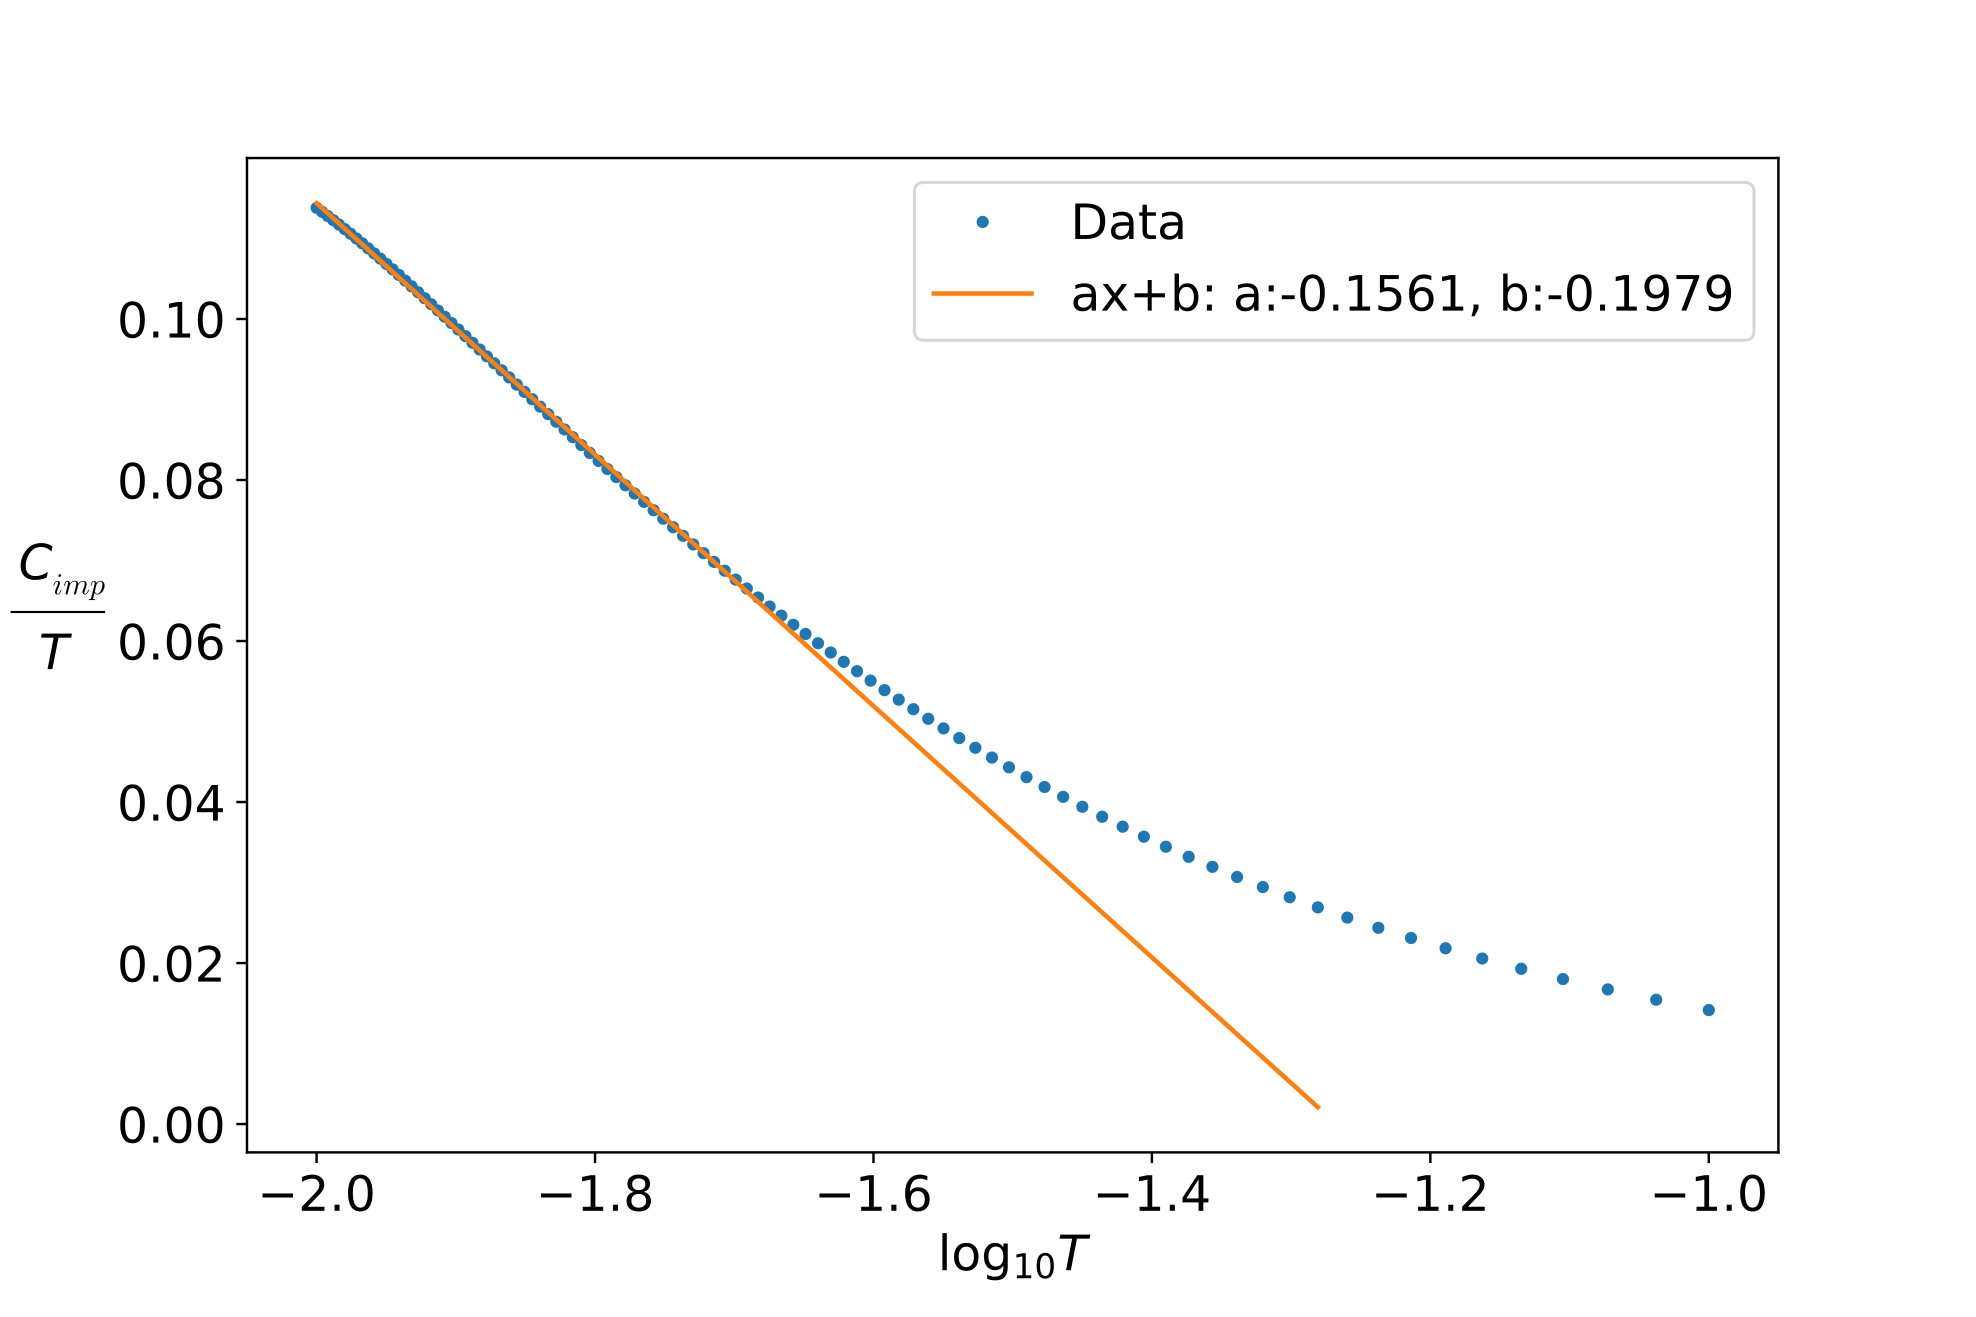
\includegraphics[width=0.7\textwidth]{plt/all/FINAL_fitted_Cv_t_0p1.png}
\caption{This figure shows the variation of the impurity specific heat with the temperature.}
\label{fig:Cv_imp}
\end{figure}
Using the self-energy obtained above, we extract the low-temperature behaviour of the impurity specific heat in the two-channel model for $t=0.1$ and $\mathcal{J}=1$, and it is shown in fig,~\ref{fig:Cv_imp}. We find that at low temperatures, the Sommerfield coefficient \(C_\text{imp}/T\) follows a logarithmic behavior for the two-channel case, which is in agreement with the results known in the literature [CITE].
\begin{eqnarray}
\frac{C_{imp}}{T} \propto \log T
\end{eqnarray}

To calculate the magnetic susceptibilty, we numerically diagonalise the low-energy effective Hamiltonain, and use the following expression:
\begin{eqnarray}
\chi &=& \beta\bigg[\frac{\sum e^{-\beta \bar{\epsilon}_{\Lambda}} \langle \bar{S}^{z2} \rangle}{\sum e^{-\beta \bar{\epsilon}_{\Lambda}} } -\frac{\sum e^{-\beta \epsilon_{\Lambda}} \langle S^{z2 }\rangle }{\sum e^{-\beta \epsilon_{\Lambda}} } \bigg] 
\end{eqnarray}
\begin{figure}[!htb]
\centering
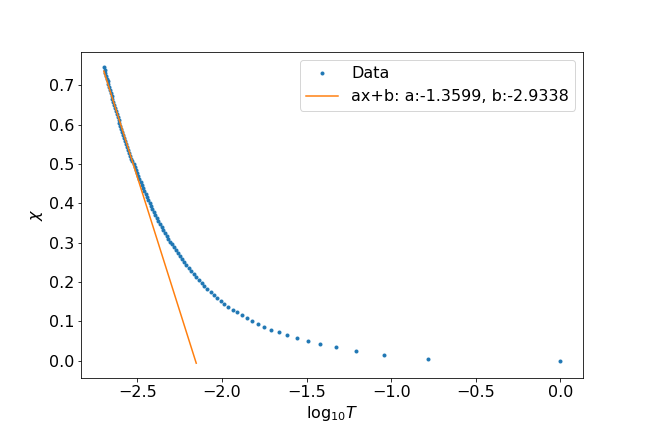
\includegraphics[width=0.7\textwidth]{plt/all/NFL_Chi_log_0p1}
\caption{Suseptibility}
\label{fig:NFL_susecptibility}
\end{figure}
The result is shown in fig.~\ref{fig:NFL_susecptibility}, and we find that at low tempertures, the suseptibility has a logarithmic behavior.
\begin{eqnarray}
\chi(T) &\propto& \log T
\end{eqnarray}

We also calculated the Wilson ratio $C_{imp}/T\chi$, and we find that taking upto three sites on each conduction channel leads to a value of $ W = 8.3$, which is greater than the known value of \(8/3\). We find that taking less number of sites leads to a lower value of \(W\), which shows that taking more number of sites will lead to a value of \(W\) that is lower than \(8.3\) and closer to \(8/3\). 

\subsection{Three channel LEH}
Similar to the two channel case, we here calculate the low energy effective Hamiltonain for three channel Kondo problem by introducing the real space hoppting on top of the zero mode three-channel stargraph model. This zero mode three channel stargraph model has three fold degenerate ground states with total $2^4=16$ states in the eigen spectrum. The three degenerate ground states are given as 
\begin{eqnarray}
|\alpha_{-1}\rangle &=& c|1000 \rangle-b (|0100 \rangle + |0010 \rangle+ | 0001 \rangle) \nonumber\\
|\alpha_{+1}\rangle &=& b(|1110 \rangle+ | 1101 \rangle + | 1011 \rangle)-c | 0111 \rangle \nonumber\\
|\alpha_0\rangle &=& -a(|1100 \rangle + |1010\rangle +|1001 \rangle)\nonumber\\
&&~~~~~~~+a(|0110 \rangle+| 0101 \rangle +| 0011\rangle)
\end{eqnarray}
where $a=0.408$, $b=0.289$, $c=0.866$. Here the state is represented by $|n_{d},n_1,n_2,n_3\rangle$, where $n_i=1/0$ represents the spin configuration $S_i^z=\pm 1/2$ respectively. Next we use degenerate perturbation theory to get the LEH which contains diagonal and off-diagonal terms. In this case we get non-zero contribution from all the three ground states $|J^z=-1\rangle$, $|J^z=0\rangle$ and $|J^z=1\rangle$. We get the diagonal contribution to the LEH in the second order to be
\begin{eqnarray}
H^{(2)}_{eff, diag} &=& - \frac{7.2 J^2}{\alpha} \hat{I}
\end{eqnarray}
The contribution associater to different ground states $|J^z=-1\rangle$, $|J^z=0\rangle$ and $|J^z=1\rangle$ is given respectively as $- \frac{2.4 J^2}{\alpha} \hat{I} + \hat{\mathcal{F}},- \frac{2.4 J^2}{\alpha} \hat{I} ,- \frac{2.4 J^2}{\alpha} \hat{I} - \hat{\mathcal{F} }$,
where $\hat{\mathcal{F}}$ is a function of diagonal number oprators of sites nearest neighbor to the zeroth site of each channels. The off-diagonal terms in the LEH is appearing due to the scattering between pair of degenerate states $(\alpha_0,\alpha_{+1})$ and $(\alpha_0,\alpha_{-1})$, there is no contribution in the second order coming from the scattering between $(\alpha_{-1},\alpha_{+1})$. The effective low energy Hamiltonian in the second ordere is given as

\begin{widetext}
\begin{eqnarray}
H^{(2)}_{eff,off-diag} &=& \sum_{\substack{(ijk)=\\(123),(231),(312)}}\bigg[ c_{i\uparrow}c_{i\downarrow}^{\dagger} \bigg( -2ab \bigg\{ \Sigma_{jk} +c_{j\uparrow}^{\dagger}c_{j\downarrow}c_{k\uparrow}c_{k\downarrow}^{\downarrow} \bigg\} -ac(\Omega_{jk}+\tilde{\Omega}_{jk}) \bigg) + ~~\textrm{h.c.}\bigg] \otimes \hat{\Xi}_l
\end{eqnarray}
\end{widetext}
where different operators are defined as
\begin{gather}
\Sigma_{i,j} = n_{i\uparrow}(1-n_{i\downarrow}) (1-n_{j\uparrow})n_{j\downarrow} + (1-n_{i\uparrow})n_{i\downarrow} n_{j\uparrow} (1 -n_{j\downarrow}), ~ ~\Omega_{i,j} =4S_i^z S_j^z n_{i\uparrow} n_{j\uparrow}, ~ ~ \tilde{\Omega}_{i,j} = 4S_{i}^zS_j^z (1-n_{i\uparrow})(1-n_{j\uparrow}) \nonumber\\
 \hat{\Xi}_l=  ( c_{l_1\uparrow}^{\dagger} c_{l_1\downarrow} +c_{l_2\uparrow}^{\dagger} c_{l_2\downarrow} + c_{l_3\uparrow}^{\dagger} c_{l_3\downarrow} + \textrm{h.c.})
\end{gather}

\section{Hamiltonian RG of spin-\(S\) impurity MCK Model}
\label{appendix_urg}
The Hamiltonian for the channel-isotropic MCK model is:
\begin{gather}
	H = \sum_l\bigg[\sum_{\substack{k\\\alpha=\uparrow,\downarrow}}\epsilon_{k,l} \hat n_{k\alpha,l} + \frac{\mathcal{J}}{2}\sum_{\substack{kk^\prime\\\alpha,\beta= \uparrow,\downarrow}} \vec{S_d}\cdot\vec{\sigma}_{\alpha\alpha^\prime}c_{k\alpha,l}^\dagger c_{k^\prime\alpha^\prime, l}\bigg]~,~~
\end{gather}
As mentioned in the same section, the Hamiltonian \(H_{(j-1)}\) of the \((j-1)^\text{th}\) RG step is obtained from the Hamiltonian \(H_{(j)}\) of the preceding RG step by applying a unitary transformation \(U_{(j)}\): \(H_{(j-1)} = U_{(j)} H_{(j)} U^\dagger_{(j)}\). The unitary transformation is obtained in terms of the fermionic operator \(\eta_{(j)}\):
\begin{gather}
	U_{(j)} = \frac{1}{\sqrt 2}\left(1 + \eta_{(j)} - \eta_{(j)}^\dagger\right)~, \\
	\hat \omega_{(j)} = H_{(j-1)} - H^i_{(j)},~T_{(j)} \equiv \text{Tr}\left(H_{(j)}c_{j}\right)~,\\
	\eta^\dagger_{(j)} = \frac{1}{\hat \omega_{(j)} - \text{Tr}\left(H_{(j)} \hat n_{j}\right) } c^\dagger_{j} T_{(j)}~.
\end{gather}
The operator \(\hat \omega_{(j)}\) encodes the quantum fluctuation scales arising from the interplay of the kinetic energy terms and the interaction terms of the Hamiltonian.

The URG equation for the single-channel Kondo model \cite{kondo_urg} shows a stable strong coupling fixed point. Ferromagnetic interactions are irrelevant. Strictly speaking, that RG equation already encodes, in principle, the multi-channel behaviour, through a modified \(\hat \omega\). To extract this information, we consider the strong coupling fixed-point \(J \gg D\) as a fixed point and analyze its stability from the star graph perspective. For the exactly-screened case, the star graph decouples from the conduction bath, leaving behind a local Fermi liquid interaction on the first site. Similarly, in the under-screened regime, the ground state is composed of states where the impurity spin is only partially screened by the conduction channels. If a particular configuration of the bath-impurity system has the total conduction bath spin down, the impurity will have a residual up spin. This induces a ferromagnetic super-exchange coupling that is irrelevant under RG, so this fixed point is stable as well. 

We now come to the over-screened case, where there is a residual spin on the conduction channel site. The neighbouring electrons will now hop in with spins opposite to that of the impurity, so an antiferromagnetic interaction will be induced, and such an interaction is relevant under the RG. This shows that the over-screened regime cannot have a stable strong coupling fixed point, and we need to search for an intermediate coupling fixed point. We therefore need the generator of the unitary transformation that incorporates third order scattering scatterings explicitly. We should take account of all possible processes that render the set of states \(\left\{\ket{\hat n_{q\beta}=1},\ket{\hat n_{q\beta}=0}\right\}\) diagonal. The higher order generator itself has two scattering processes, such that the entire renormalisation term \(c^\dagger_{q\beta} T \eta\) has in total three coherent processes. The complete generator upto third order can be written as
\begin{widetext}
\begin{equation}\begin{aligned}
	\eta = \frac{1}{\hat \omega - H_D}T^\dagger c \simeq \frac{1}{\omega^\prime - H_D}T^\dagger c + \frac{1}{\omega^\prime - H_D}H_X \frac{1}{\omega^\prime - H_D} T^\dagger c + \frac{1}{\omega^\prime - H_D} T^\dagger c \frac{1}{\omega^\prime - H_D} H_X
\end{aligned}\end{equation}
where \(H_X = J \sum_{k,k^\prime < \Lambda_j, \alpha,\alpha^\prime}\vec{S_d}\cdot\vec{s}_{\alpha \alpha^\prime}c^\dagger_{k\alpha}c_{k^\prime\alpha^\prime}\) is scattering between the entangled electrons. There are two third order terms in the above equation corresponding to the two possible sequences in which the processes can occur while keeping the total renormalisation \(c^\dagger_{q\beta}T \eta\) diagonal in \(q\beta\). The second order processes remain unchanged. The total renormalisation takes the form:
\begin{equation}
	\label{full_ren}
	\Delta H_{(j)} = \underbrace{c^\dagger T \frac{1}{\omega^\prime - H_D} T^\dagger c  + \left(c^\dagger \leftrightarrow c\right)}_{\Delta H^{(2)}_{(j)}} + \underbrace{c^\dagger T \frac{1}{\omega^\prime - H_D} H_X \frac{1}{\omega^\prime - H_D} T^\dagger c + c^\dagger T \frac{1}{\omega^\prime - H_D} T^\dagger c \frac{1}{\omega^\prime - H_D} H_X + \left(c^\dagger \leftrightarrow c\right)}_{\Delta H^{(3)}_{(j)}}
\end{equation}
\(\Delta H^{(2)}_{(j)}\) and \(\Delta H^{(3)}_{(j)}\) are the renormalisation arising from the the second and third order processes respectively.

It is easier to see the RG flow of the couplings if we write the Hamiltonian in terms of the eigenstates of \(S_d^z\). These eigenstates are defined by \(S_d^z\ket{m_d} = m_d\ket{m_d}, m_d \in \left[-S, S\right]\). In terms of these eigenstates, the Hamiltonian becomes
\begin{equation}\begin{aligned}
	\label{H_spin_S}
	\mathcal{H} = \sum_{k\sigma}\epsilon_{k}\tau_{k\sigma} + \sum_{m_d=-S}^S \sum_{kl,\atop{\sigma=\uparrow,\downarrow}} J^\sigma_{m_d} \ket{m_d}\bra{m_d} c^\dagger_{k \sigma}c_{l \sigma} + \sum_{kl} \sum_{m_d=-S}^{S-1} J^t_{m_d} \left(\ket{m_d+1}\bra{m_d} s^-_{kl}  + \text{h.c.}\right)
\end{aligned}\end{equation}
\end{widetext}
where \(k,l\) sum over the momentum states, \(\sigma\) sums over the spin indices, \(J^\sigma_m = \frac{1}{2} \sigma m J\) in the UV Hamiltonian, and \(J^t_{m} = J\frac{1}{2}\sqrt{S(S+1) - m(m+1)}\) is the coupling that connects \(\ket{m}\) and \(\ket{m+1}\). We first calculate \(\Delta H^{(2)}_{(j)}\). There will be two types of processes - those processes that start from an occupied state (particle sector) and those that start from a vacant state (hole sector). Due to particle hole symmetry of the Hamiltonian, they will be equal to each other and we will only calculate the particle sector contribution. 

In the particle sector, we have (\(\hat n_{q\beta}=1\)), so we will work at a negative energy  shell \(\epsilon_q = -D\). The renormalisation can schematically represented as \(H^I_0 \frac{1}{\omega - H^D_{q\beta}} H^I_1\). Both \(H^I_0\) and \(H^I_1\) have all three operators \(S_d^z, S_d^\pm\). We first consider specifically the case of spin-\(\frac{1}{2}\) impurity. Those terms that have identical operators on both sides can be ignored because \({S_d^z}^2 = \text{constant}\) and \({S^\pm}^2 = 0\). All the six terms that \textit{will} renormalise the Hamiltonian have a spin flip operator on at least one side of the Greens function. This means that in the denominator of the Greens function, \(S_d^z\) and \(s^z_{qq}\) have to be anti-parallel in order to produce a non-zero result for that term. This means we can identically replace \(S_d^z s^z_{qq} = -\frac{1}{4}\). Also, in the particle sector, the Greens function always has \(c_{q\beta}\) in front of it, so \(\epsilon_q \tau_{q\beta} = \frac{D}{2}\). The upshot of all this is that the denominator of all scattering processes for the spin-\(\frac{1}{2}\) impurity Hamiltonian will be \(\omega - \frac{D}{2} + \frac{J}{4}\).

We now come to the general case of spin-\(S\) impurity. The various terms that renormalise the Hamiltonian can be described in terms of the bath spin operators that come into them. For example, the term that has \(s^z\) on both sides of the intervening Greens function can be represented as \(z|z\). There are 7 such terms: \(z|z, \pm|\mp, z|\pm, \pm|z\). Each of these terms occur both in the particle and the hole sectors. We will demonstrate the calculation of two of these terms. The \(z|z\) \(+|-\) terms evaluate in the following manner.
\begin{widetext}
\begin{align}
	z|z: & \sum_{kk^\prime,m,\sigma} c^\dagger_{q \sigma} c_{k^\prime \sigma} \ket{m}\bra{m}\frac{{J^\sigma_m}^2}{\omega - \frac{D}{2} + \frac{J}{2}\sigma S_d^z}\ket{m}\bra{m} c^\dagger_{k \sigma}c_{q \sigma} = -\sum_{kk^\prime,m,\sigma}n_{q \sigma}\frac{{J^\sigma_m}^2 c^\dagger_{k \sigma}c_{k^\prime\sigma} \ket{m}\bra{m}}{\omega_{m, \sigma} - \frac{D}{2} + \frac{J}{2}\sigma m}\\
	+|-: & \sum_{kk^\prime,m} c^\dagger_{q \uparrow} c_{k^\prime \downarrow} \ket{m}\bra{m+1}\frac{{J^t_m}^2}{\omega - \frac{D}{2} + \frac{J}{2}S_d^z}\ket{m+1}\bra{m} c^\dagger_{k \downarrow}c_{q \uparrow} = -n_{q \uparrow}\sum_{kk^\prime,m}\frac{{J^t_m}^2 c^\dagger_{k \downarrow}c_{k^\prime\downarrow} \ket{m}\bra{m}}{\omega_{m+1, \uparrow} - \frac{D}{2} + \frac{J}{2}\left( m+1 \right) }
\end{align}
\end{widetext}
We similarly compute the rest of the terms. We again define \(\sum_q \hat n_{q\sigma} = n(D)\). To compare with the spin-\(\frac{1}{2}\) RG equations, we will transform the general spin-\(S\) \(\omega\) to the spin-\(\frac{1}{2}\) \( \omega\), using \(\omega_{m,\sigma} \to \omega - \frac{J}{2}\left(m\sigma - \frac{1}{2}\right)\).

The renormalisation in \(J^\sigma_m\) is
\begin{equation}\begin{aligned}
	\Delta J^\sigma_{m} = - n(D) \frac{\left( J^\sigma_m \right) ^2 + \left( J^t_{m-\frac{1+\sigma}{2}} \right) ^2}{\omega - \frac{D}{2} + \frac{J}{4}}~.
\end{aligned}\end{equation}
Here, we have defined \(J^t_m = 0\) for \( |m| > S\). Two relations can be obtained from this RG equation, the RG equations for the sum and difference of the couplings: \(J^\pm_m = \frac{1}{2}\left(J^\uparrow_m \pm J^\downarrow_m\right) \). The RG equation for the sum of the couplings is
\begin{equation}\begin{aligned}
	\Delta J^+_m = -n(D)\frac{\sum_\sigma \left( J^\sigma_m \right) ^2 + \sum_\sigma \left( J^t_{m-\frac{1+\sigma}{2}} \right) ^2}{2\left(\omega - \frac{D}{2} + \frac{J}{4}\right)}\\
	= -n(D)\frac{J^2}{4}\frac{S(S+1)}{\omega - \frac{D}{2} + \frac{J}{4}}
\end{aligned}\end{equation}
This is an \(m-\)independent piece, so it can be summed over to produce an impurity-independent potential scattering term, which we ignore. 

The second is the RG equation for the difference of the couplings:
\begin{equation}\begin{aligned}
	\Delta J^-_m = -n(D)\frac{1}{2}\frac{\left( J^t_{m-1} \right) ^2 - \left(J^t_{m}\right) ^2}{\omega - \frac{D}{2} + \frac{J}{4}} = -\frac{1}{4}\frac{n(D) m J^2}{\omega - \frac{D}{2} + \frac{J}{4}}
\end{aligned}\end{equation}
The usual \(J\) Kondo coupling is recovered through \(J = 2J^-_m/m\). Substituting this gives 
\begin{equation}\begin{aligned}
	\Delta_\text{p sector} J = -\frac{1}{2}n(D)\frac{J^2}{\omega - \frac{D}{2} + \frac{J}{4}}
\end{aligned}\end{equation}

We can also obtain the RG equation for \(J\) from the transverse renormalisation:
\begin{equation}\begin{aligned}
	\Delta J^t_m &= - \frac{n(D)J^t_m \left( J^\downarrow_m + J^\uparrow_{m+1} \right) }{\omega - \frac{D}{2} + \frac{J}{4}} = -\frac{1}{2}\frac{n(D)J^t_m J}{\omega - \frac{D}{2} + \frac{J}{4}}
\end{aligned}\end{equation}
Since \(J^t_m \propto J\), we have
\begin{equation}\begin{aligned}
	\Delta J_\text{p sector} &= -\frac{1}{2}\frac{n(D)J^2}{\omega - \frac{D}{2} + \frac{J}{4}}
\end{aligned}\end{equation}
The total renormalisation from both particle and hole sectors, at this order, is
\begin{equation}\begin{aligned}
	\Delta J^{(2)} &= -\frac{n(D)J^2}{\omega - \frac{D}{2} + \frac{J}{4}}
\end{aligned}\end{equation}

We now come to the third order renormalisation.
Following eq.~\ref{full_ren}, the next order renormalisation is
\begin{equation}\begin{aligned}
	\label{psector_3rd_ren}
	\Delta H^{(3)}_j = c^\dagger T \frac{1}{\omega^\prime - H_D} H_X \frac{1}{\omega^\prime - H_D} T^\dagger c \\
	+ c^\dagger T \frac{1}{\omega^\prime - H_D} T^\dagger c \frac{1}{\omega^\prime - H_D} H_X
\end{aligned}\end{equation}
The first term will be of the form
\begin{widetext}
\begin{equation}\begin{aligned}
	\sum_{q,k,l_1} c^\dagger_{q\beta, l_1}c_{k \alpha, l_1}\ket{m_1}\bra{m_2} \frac{1}{\omega - \frac{D}{2} - \frac{\epsilon_k}{2} + \frac{\beta J}{4}S_d^z} \ket{m_2} c^\dagger_{k_1 \sigma_1, l_2}c_{k_2 \sigma_2,l_2} \bra{m_3}\frac{1}{\omega - \frac{D}{2} - \frac{\epsilon_k}{2} + \frac{\beta J}{4}S_d^z}\ket{m_3}\bra{m_4}c^\dagger_{k\alpha, l_1}c_{q\beta, l_1}
\end{aligned}\end{equation}
\end{widetext}
We have not bothered to write all the summations and the couplings correctly, because we will only simplify the denominator here. Evaluating the inner products gives
\begin{equation}\begin{aligned}
	\sum_{qk,l_1} \frac{\ket{m_1}\bra{m_4}c^\dagger_{q\beta}c_{k \alpha}c^\dagger_{k_1 \sigma_1, l_2}}{\omega_{m_2,\beta} - \frac{D}{2} - \frac{\epsilon_k}{2} + \frac{\beta J m_2}{4}}  \frac{c_{k_2 \sigma_2,l_2}c^\dagger_{k\alpha}c_{q\beta}}{\omega_{m_3,\beta} - \frac{D}{2} - \frac{\epsilon_k}{2} + \frac{\beta J m_3}{4}}
\end{aligned}\end{equation}
We again use \(\omega_{m,\sigma} \to \omega - \frac{J}{2}\left(m\sigma - \frac{1}{2}\right)\).
\begin{equation}\begin{aligned}
	\ket{m_1}\bra{m_4}c^\dagger_{k_1 \sigma_1, l_2}c_{k_2 \sigma_2,l_2}\sum_{qk,l_1} \frac{\hat n_{q\beta}\left(1 - \hat n_{k\alpha}\right)}{\left(\omega - \frac{D}{2} - \frac{\epsilon_k}{2} + \frac{J}{4}\right)^2}
\end{aligned}\end{equation}
We define \(\sum_q \hat n_{q\beta} = n(D)\). Performing the sums over \(k\) and \(l_1\) gives
\begin{equation}\begin{aligned}
	-\frac{1}{2}\ket{m_1}\bra{m_4}c^\dagger_{k_1 \sigma_1, l_2}c_{k_2 \sigma_2,l_2} \frac{\rho n(D) K}{\omega - \frac{D}{2} + \frac{J}{4}}
\end{aligned}\end{equation}
\(\rho\) is the density of states which we have taken to be constant. Reinstating the complete summation and the couplings gives
\begin{equation}\begin{aligned}
	\label{first_group}
	-\frac{1}{2}\frac{\rho n(D) K}{\omega - \frac{D}{2} + \frac{J}{4}}\sum_{m_1,m_4,k_1,k_2,\atop{l_2,\sigma_1\sigma_2}}\lambda_{1}\lambda_{2}\lambda_{3}\ket{m_1}\bra{m_4}c^\dagger_{k_1 \sigma_1, l_2}c_{k_2 \sigma_2,l_2}
\end{aligned}\end{equation}
There is no sum over \(m_2\) and \(m_3\) because they are constrained by \(m_1\) and \(m_4\) respectively. \(\lambda_i\) represent the couplings present at the three interaction vertices. \(k_{1,2}\) sum over the momenta, \(\sigma_{1,2}\) sum over the spin indices and \(l_2\) sums over the channels.

The second term in eq.~\ref{psector_3rd_ren} can be evaluated in an almost identical fashion. The integral here be negative of the first term, because of an exchange in the scattering processes.
\begin{equation}\begin{aligned}
	\label{second_group}
	\frac{1}{2}\frac{\rho n(D) K}{\omega - \frac{D}{2} + \frac{J}{4}}\sum_{m_1,m_4,k_1,k_2,\atop{l_2,\sigma_1\sigma_2}}\lambda_{1}\lambda_{3}\lambda_{2}\ket{m_1}\bra{m_4}c^\dagger_{k_1 \sigma_1, l_2}c_{k_2 \sigma_2,l_2}
\end{aligned}\end{equation}

The first group of terms (those that appear in \ref{first_group}) in the particle sector can be represented as \(a|b^\prime|c\), where \(a,b,c \in \left\{z,+,-\right\} \) and represent the operator for the conduction electrons in the three ceonnected processes. The \(\prime\) on \(b\) indicates that it is the state of the electrons \textit{not being decoupled}. The second group of terms (those that appear in \ref{second_group}) are therefore represented as \(a|b|c^\prime\), because in this group, the interaction \(H_X\) between the electrons that are not being decoupled occur at the very end.
We will only calculate the terms in the particle sector, the ones in hole sector will be equal to these because of particle-hole symmetry. The full list of terms is: 
$z|z^\prime|z\quad$
$z|z|z^\prime\quad$
$-|z^\prime|+\quad$
$-|+|z^\prime\quad$
$+|z^\prime|-\quad$
$+|-|z^\prime\quad$
$ z|+^\prime|z\quad$
$z|-^\prime|z\quad$
$+|+^\prime|-\quad$
$-|+^\prime|+\quad$
$z|z|+^\prime\quad$
$z|z|-^\prime\quad$
$ +|-|+^\prime\quad$
$+|-|-^\prime\quad$
$-|+|+^\prime\quad$
$z|z^\prime|z\quad$
$z|z|z^\prime\quad$
$-|z^\prime|+\quad$
$ -|+|z^\prime\quad$
$+|z^\prime|-\quad$
$+|-|z^\prime\quad$
$z|+^\prime|z\quad$
$z|-^\prime|z\quad$
$+|+^\prime|-\quad$
$-|+^\prime|+\quad$
$z|z|+^\prime\quad$
$z|z|-^\prime\quad$
$+|-|+^\prime\quad$
$+|-|-^\prime\quad$
$-|+|+^\prime\quad$
.

The total renormalisation in  \(J^\sigma_m\) is
\begin{widetext}
\begin{equation}\begin{aligned}
	\Delta J^\sigma_m = \frac{1}{2}\frac{\rho n(D) K}{\omega - \frac{D}{2} + \frac{J}{4}}\left[\left( J^t_{m-1} \right)^2 J^\sigma_m + \left( J^t_m \right)^2 J^\sigma_m - \left( J^t_{m-1} \right)^2 J^\sigma_{m-1} - \left(J^t_m\right)^2 J^\sigma_{m+1} \right] = \frac{1}{2}\frac{\rho n(D) K}{\omega - \frac{D}{2} + \frac{J}{4}}J^3 m \sigma
\end{aligned}\end{equation}
Since we had defined \(J^\sigma_m \equiv \frac{1}{2}J m \sigma\), we have \(\Delta J = \frac{2}{m\sigma}\Delta J^\sigma_m\), and we get \(\Delta_\text{p sector} J = \frac{1}{4}\frac{\rho n(D) K}{\omega - \frac{D}{2} + \frac{J}{4}}J^3\).
Combining with the hole sector renormalisation, we get
\begin{equation}\begin{aligned}
	\Delta J^{(3)} = \frac{1}{2}\frac{\rho n(D) K}{\omega - \frac{D}{2} + \frac{J}{4}}J^3
\end{aligned}\end{equation}
The total renormalisation in \(J\) after combining all orders is
\begin{equation}\begin{aligned}
	\Delta J = -\frac{n(D) J^2}{\omega - \frac{D}{2} + \frac{J}{4}} + \frac{1}{2}\frac{\rho n(D) K}{\omega - \frac{D}{2} + \frac{J}{4}}J^3
\end{aligned}\end{equation}
\end{widetext}

\bibliography{mscript_mck_full}
\end{document}
